\documentclass{cisXXX}

\HWauthor[Simone Rinaldi]{Simone Rinaldi (matr. 737270)}{s.rinaldi012@studenti.unibs.it}
\HWauthor[Matteo Legati]{Matteo Legati (matr. 735612)}{m.legati002@studenti.unibs.it}
\HWcourse{Algoritmi e Strutture Dati}
\HWtitle[Problema dell'ingaggio dei giocatori svincolati]{Signing Free-Agent Baseball Players}
\date{Elaborato a.a. 2025/26 \\[0.3em] Prof.ssa Marina Zanella}

\usepackage[utf8]{inputenc}
\usepackage[T1]{fontenc}
\usepackage{lmodern}
\usepackage[italian]{babel}
\usepackage{amsmath}
\usepackage{amssymb}
\usepackage{graphicx}
\usepackage{booktabs}
\usepackage{microtype}
\usepackage{xcolor}
\usepackage{algorithm}
\usepackage{algpseudocode}
\usepackage{listings}
\usepackage[colorlinks=true, linkcolor=blue!70!black, citecolor=blue!70!black, urlcolor=blue!70!black]{hyperref}

% Configurazione listings per codice Python
\lstset{
	language=Python,
	basicstyle=\ttfamily\footnotesize,
	keywordstyle=\color{blue!80!black}\bfseries,
	commentstyle=\color{gray!80!black}\textit,
	stringstyle=\color{teal},
	numbers=left,
	numberstyle=\tiny\color{gray},
	stepnumber=1,
	numbersep=6pt,
	backgroundcolor=\color{gray!6},
	frame=single,
	rulecolor=\color{gray!30},
	tabsize=4,
	showstringspaces=false,
	breaklines=true
}

% Configurazione stile pseudocodice
\algrenewcommand\algorithmicrequire{\textbf{Input:}}
\algrenewcommand\algorithmicensure{\textbf{Output:}}
\algrenewcommand{\algorithmiccomment}[1]{\hfill\textcolor{gray!80!black}{\textit{// #1}}}

\graphicspath{{figures/}{../results/}}

\begin{document}
\maketitle

\newpage

\tableofcontents

\vfil

\section{Modellazione e Algoritmi Fondamentali}

\subsection{Descrizione del Problema e Formulazione Matematica}
Per questo elaborato è stato scelto il problema dell'ingaggio dei giocatori svincolati (\textit{Signing Free-Agent Baseball Players}). Trae la propria formulazione canonica dal Problema~14-12 del testo di Cormen et al.\footnote{T.~H.~Cormen, C.~E.~Leiserson, R.~L.~Rivest, C.~Stein, \textit{Introduction to Algorithms}, 4th ed., MIT Press, Cambridge, MA, 2022.}. Nel dominio dell'ottimizzazione combinatoria, si configura come un'istanza del \textit{Multiple-Choice Knapsack Problem} (MCKP), variante del classico problema dello zaino in cui l'insieme degli oggetti selezionabili è partizionato in classi disgiunte e mutualmente esclusive. Lo scenario decisionale modella l'obiettivo della dirigenza di una squadra sportiva che, a fronte di un budget finanziario prefissato, mira a massimizzare la competitività globale della formazione ingaggiando atleti sul mercato degli \textit{svincolati}, nel rispetto del vincolo di copertura dei ruoli e del tetto massimo di budget spendibile.

Formalmente, un'istanza del problema è definita da un budget finanziario nominale $X \in \mathbb{R}^+$, da un insieme di $N$ ruoli (indicizzati con $i \in \{1, \dots, N\}$, dove nel contesto del baseball si assumono i canonici $N = 9$ ruoli difensivi) e da una collezione di $P$ candidati svincolati disponibili per ciascun ruolo (indicizzati con $k \in \{1, \dots, P\}$). Ciascun candidato è univocamente caratterizzato da un compenso contrattuale nominale $\mathit{cost}_{i,k}^{\text{nom}} \in \mathbb{R}^+$ e da una misura quantitativa di rendimento tecnico $\mathit{war}_{i,k} \ge 0$, espressa tramite la statistica \textbf{WAR} (\textit{Wins Above Replacement}).

Per specifica di progetto, i compensi monetari sono espressi come multipli interi di una costante di discretizzazione $\text{COST\_UNIT} = 100\,000$. È pertanto possibile ricondurre l'istanza a una formulazione intera esatta definendo il budget discreto $B = \lfloor X / \text{COST\_UNIT} \rfloor$ e i corrispondenti costi interi scalati $\mathit{cost}_{i,k} = \lfloor \mathit{cost}_{i,k}^{\text{nom}} / \text{COST\_UNIT} \rfloor$.

Associando a ciascun candidato una variabile di decisione binaria $x_{i,k} \in \{0, 1\}$, indicante se il candidato $k$ del ruolo $i$ viene ingaggiato ($x_{i,k} = 1$) o meno ($x_{i,k} = 0$), il problema si formalizza come segue:
\begin{align}
	\max \quad              & \sum_{i=1}^N \sum_{k=1}^P \mathit{war}_{i,k} \, x_{i,k} \label{eq:objective}                                                     \\
	\text{soggetto a} \quad & \sum_{k=1}^P x_{i,k} \le 1 \quad \forall i \in \{1, \dots, N\} \label{eq:constraint_roster}                           \\
	                        & \sum_{i=1}^N \sum_{k=1}^P \mathit{cost}_{i,k} \, x_{i,k} \le B \label{eq:constraint_budget}                                       \\
	                        & x_{i,k} \in \{0, 1\} \quad \forall i \in \{1, \dots, N\}, \; \forall k \in \{1, \dots, P\} \label{eq:constraint_binary}
\end{align}
Il vincolo~\eqref{eq:constraint_roster} impone l'esclusività di ruolo (al massimo un acquisto per posizione), il vincolo~\eqref{eq:constraint_budget} garantisce il rispetto del tetto di spesa complessivo $B$, mentre la funzione obiettivo~\eqref{eq:objective} massimizza il WAR complessivo della rosa. La risoluzione dell'istanza richiede di determinare sia il valore scalare ottimo conseguibile, sia l'esatta configurazione della rosa che lo realizza, corredata dal costo cumulativo effettivo.

\subsection{Applicabilità della Programmazione Dinamica}
L'applicabilità del paradigma della programmazione dinamica a un problema di ottimizzazione poggia su due presupposti teorici necessari: la presenza di una \textit{sottostruttura ottima} e la presenza di \textit{sottoproblemi sovrapposti} (\textit{overlapping subproblems}).

\subsubsection{Definizione dei Sottoproblemi}
Per formulare lo spazio degli stati, decomponiamo il problema originale considerando prefissi dell'insieme dei ruoli e quote parziali di bilancio. Definiamo formalmente il generico \textbf{sottoproblema} associato alla coppia di indici $(i, b)$ come:
\begin{quote}
	\textit{«Massimizzare il WAR complessivo considerando esclusivamente un sottoinsieme di ruoli compresi tra i primi $i$ ($0 \le i \le N$), disponendo di una quantità di budget residuo non superiore a $b$ ($0 \le b \le B$).»}
\end{quote}
Indichiamo con $m[i, b]$ il valore della soluzione ottima per tale sottoproblema. Il problema originario corrisponde alla valutazione dello stato terminale $m[N, B]$.

\subsubsection{Dimostrazione della Sottostruttura Ottima}
Un problema esibisce una sottostruttura ottima se una soluzione ottima al problema contiene al proprio interno soluzioni ottime per i relativi sottoproblemi. Dimostriamo tale proprietà conducendo una dimostrazione per assurdo.

Sia $R^*$ una soluzione ottima per il sottoproblema generico $(i, b)$, ovvero una selezione ammissibile di candidati tra i primi $i$ ruoli che rispetta la spesa cumulativa $\le b$ e ottiene il rendimento massimo $m[i, b]$. Rispetto alla decisione adottata per l'$i$-esimo ruolo, si distinguono due casi mutualmente esclusivi ed esaustivi:
\begin{enumerate}
	\item \textbf{Caso 1: Nessun candidato viene ingaggiato per il ruolo $i$.} \\
	      In questo caso la rosa $R^*$ impiega unicamente giocatori appartenenti ai primi $i-1$ ruoli con una spesa complessiva non superiore a $b$. Di conseguenza, $R^*$ costituisce una soluzione ammissibile per il sottoproblema $(i-1, b)$. Se per assurdo $R^*$ non fosse ottima per $(i-1, b)$, esisterebbe una rosa ammissibile $R'$ sui primi $i-1$ ruoli, con spesa $\le b$, tale che $\text{WAR}(R') > \text{WAR}(R^*)$. Poiché $R'$ non alloca alcun giocatore al ruolo $i$, essa risulterebbe ammissibile anche per $(i, b)$ con rendimento $\text{WAR}(R') > \text{WAR}(R^*)$, contraddicendo l'ipotesi di ottimalità globale di $R^*$ su $(i, b)$. Pertanto, $R^*$ deve essere ottima per $(i-1, b)$.

	\item \textbf{Caso 2: Viene ingaggiato il candidato $p$ per il ruolo $i$, avente costo scalato $\mathit{cost}_{i, p} \le b$ e rendimento $\mathit{war}_{i, p}$.} \\
	      Sottraendo $p$ dalla soluzione ottima, consideriamo la sottorosa residua $R' = R^* \setminus \{p\}$. Poiché la spesa complessiva di $R^*$ è limitata da $b$, la spesa impegnata da $R'$ sui primi $i-1$ ruoli non eccede $b - \mathit{cost}_{i, p}$; inoltre, la separazione dei ruoli garantisce che $R'$ contenga al più un giocatore per ciascuna delle prime $i-1$ posizioni. Dunque, $R'$ è ammissibile per il sottoproblema $(i-1, b - \mathit{cost}_{i, p})$, con rendimento pari a $\text{WAR}(R') = \text{WAR}(R^*) - \mathit{war}_{i, p}$. \\
	      Se per assurdo $R'$ non fosse ottima per $(i-1, b - \mathit{cost}_{i, p})$, esisterebbe una configurazione ammissibile alternativa $R''$ sui primi $i-1$ ruoli avente costo $\le b - \mathit{cost}_{i, p}$ e rendimento strettamente superiore: $\text{WAR}(R'') > \text{WAR}(R')$.
	      Sostituendo $R'$ con $R''$ e reintroducendo il candidato $p$, costruiamo la nuova rosa $R_{\text{new}} = R'' \cup \{p\}$. Tale rosa rispetta il vincolo di ruolo (include $p$ al ruolo $i$ e al più un giocatore per ciascuno dei primi $i-1$ ruoli) e il vincolo finanziario, poiché la spesa totale risulta $\le (b - \mathit{cost}_{i, p}) + \mathit{cost}_{i, p} = b$. Il rendimento complessivo ottenuto è:
	      \[
		      \text{WAR}(R_{\text{new}}) = \text{WAR}(R'') + \mathit{war}_{i, p} > \text{WAR}(R') + \mathit{war}_{i, p} = \text{WAR}(R^*)
	      \]
	      La configurazione ammissibile $R_{\text{new}}$ conseguirebbe un WAR strettamente superiore a quello della soluzione ottima $R^*$, generando una contraddizione. Ne consegue che la sottorosa $R'$ deve essere una soluzione ottima per il sottoproblema $(i-1, b - \mathit{cost}_{i, p})$.
\end{enumerate}
In entrambi i casi, la soluzione ottima globale incorpora soluzioni ottime per i rispettivi sottoproblemi, certificando la validità della proprietà di sottostruttura ottima.

\subsubsection{Sovrapposizione dei Sottoproblemi}
La seconda condizione per l'efficacia della programmazione dinamica è l'esistenza di sottoproblemi comuni ricorsivamente condivisi. Lo spazio di tutti i possibili sottoproblemi distinti è circoscritto alla griglia discreta degli indici $(i, b)$, per un totale complessivo di $(N + 1) \times (B + 1)$ stati.

Un approccio ricorsivo ingenuo privo di memorizzazione compirebbe a ogni livello $i$ una diramazione su $P + 1$ scelte alternative (non ingaggiare nessuno o selezionare uno tra i $P$ candidati), sviluppando un albero di ricorsione di profondità $N$ con una complessità temporale nell'ordine di $\Omega((P + 1)^N)$, computazionalmente intrattabile anche per istanze di modesta entità. Tuttavia, sequenze distinte di decisioni sui primi ruoli confluiscono frequentemente nel medesimo stato residuo $(i, b)$: allocazioni finanziarie differenti ma equivalenti in termini di spesa cumulata portano allo stesso budget residuo per i ruoli successivi. Memorizzando sistematicamente i risultati parziali in una struttura dati tabellare, ciascun sottoproblema viene risolto una sola volta, consentendo consultazioni in tempo costante $\Theta(1)$ ed eliminando l'esplosione combinatoria dell'albero di decisione.

\subsubsection{Equazione di Ricorrenza}
In virtù delle proprietà dimostrate, il valore $m[i, b]$ della soluzione ottima per lo stato $(i, b)$ è calcolabile mediante la seguente equazione di ricorrenza di Bellman:
\begin{equation}
	m[i, b] = \begin{cases}
		0 & \text{se } i = 0 \text{ oppure } b = 0                       \\
		\max \left( m[i - 1, b], \; \max\limits_{\substack{1 \le k \le P \\ \mathit{cost}_{i, k} \le b}} \{ m[i - 1, b - \mathit{cost}_{i, k}] + \mathit{war}_{i, k} \} \right) & \text{se } i > 0 \text{ e } b > 0
	\end{cases}
	\label{eq:bellman}
\end{equation}
Il caso base stabilisce che, in assenza di ruoli disponibili ($i = 0$) o in assenza di budget ($b = 0$), nessun ingaggio incrementale è consentito, attestando il WAR a $0.0$. Nel passo ricorsivo, il primo termine dell'operatore $\max$ esprime la scelta conservativa di non effettuare alcun ingaggio al ruolo $i$, preservando il rendimento $m[i-1, b]$ conseguito sui ruoli precedenti senza assorbire budget. Il secondo termine valuta l'ingaggio di ciascun candidato ammissibile $k \in \{1, \dots, P\}$ avente costo $\mathit{cost}_{i,k} \le b$, sommando il rispettivo valore $\mathit{war}_{i, k}$ all'ottimo del sottoproblema residuo $m[i - 1, b - \mathit{cost}_{i, k}]$.

\subsection{Algoritmi Risolutivi e Pseudocodici}
Il processo risolutivo è articolato in due procedure complementari:
la procedura \textsc{Compute-Optimal-War} (Algoritmo~\ref{alg:compute_optimal_war}), che calcola il valore scalare ottimo popolando la tabella dinamica $m$ e registrando le scelte di transizione nella tabella ausiliaria $s$;
la procedura \textsc{Reconstruct-Optimal-Roster} (Algoritmo~\ref{alg:reconstruct_optimal_roster}), che risale la tabella delle decisioni a ritroso per isolare l'elenco dei giocatori effettivamente ingaggiati e il costo totale sostenuto.

\subsubsection{Calcolo del Valore Ottimo e Tracciamento delle Scelte}
L'Algoritmo~\ref{alg:compute_optimal_war} implementa un approccio \textit{bottom-up} iterativo. Vengono allocate due matrici di dimensione $(N + 1) \times (B + 1)$: la tabella $m$, inizializzata a $0.0$, destinata a contenere i massimi valori di WAR per ogni sottoproblema, e la tabella $s$, inizializzata a $-1$, impiegata per registrare l'indice del candidato selezionato per ciascuno stato (convenzionalmente $-1$ indica la mancata acquisizione nel ruolo corrente).

Per ogni ruolo, la riga corrente viene inizialmente copiata dalla riga precedente ($m[i, b] \gets m[i-1, b]$), incorporando la decisione di base (nessun acquisto). Successivamente, si esamina ciascun candidato $j \in \{0, \dots, P - 1\}$: per ogni livello di budget $b \ge c$, viene valutato l'eventuale ingaggio del giocatore; qualora produca un rendimento strettamente superiore al valore corrente $m[i, b]$, la cella viene aggiornata e l'indice $j$ viene memorizzato in $s[i, b]$. Al termine dell'esecuzione, la cella $m[N, B]$ contiene il valore ottimo globale.

\begin{algorithm}[H]
	\small
	\caption{Calcolo del WAR Ottimale e della Tabella delle Scelte}
	\label{alg:compute_optimal_war}
	\begin{algorithmic}[1]
		\Require Numero di ruoli $N \in \mathbb{N}$, budget nominale $X \in \mathbb{R}^+$, candidati per ruolo $P \in \mathbb{N}$, matrice $\mathit{players}[0 \dots N-1, 0 \dots P-1]$
		\Ensure Valore ottimo $\mathit{optimal\_war} \in \mathbb{R}^+$, matrice delle decisioni $s[0 \dots N, 0 \dots B]$
		\Procedure{Compute-Optimal-War}{$N, X, P, \mathit{players}$}
		\State $\text{COST\_UNIT} \gets 100\,000$
		\State $B \gets \lfloor X / \text{COST\_UNIT} \rfloor$
		\State alloca $m[0 \dots N, 0 \dots B]$ inizializzata a $0.0$
		\State alloca $s[0 \dots N, 0 \dots B]$ inizializzata a $-1$
		\For{$i \gets 1$ \textbf{to} $N$} \Comment{Iterazione sugli stadi decisionali (ruoli)}
		\State $m[i, 0 \dots B] \gets m[i - 1, 0 \dots B]$ \Comment{Scelta base: nessun ingaggio al ruolo $i$}
		\For{$j \gets 0$ \textbf{to} $P - 1$} \Comment{Valutazione dei candidati disponibili}
		\State $p \gets \mathit{players}[i - 1, j]$
		\State $c \gets \lfloor p.\mathit{cost} / \text{COST\_UNIT} \rfloor$
		\For{$b \gets c$ \textbf{to} $B$} \Comment{Aggiornamento degli stati con budget sufficiente}
		\State $\mathit{war} \gets m[i - 1, b - c] + p.\mathit{war}$
		\If{$\mathit{war} > m[i, b]$}
		\State $m[i, b] \gets \mathit{war}$
		\State $s[i, b] \gets j$ \Comment{Tracciamento della scelta ottima}
		\EndIf
		\EndFor
		\EndFor
		\EndFor
		\State \textbf{return} $m[N, B], \; s$
		\EndProcedure
	\end{algorithmic}
\end{algorithm}

\subsubsection{Ricostruzione della Rosa Ottima}
La procedura \textsc{Reconstruct-Optimal-Roster} (Algoritmo~\ref{alg:reconstruct_optimal_roster}) prende in ingresso la matrice delle decisioni $s$ e ricostruisce la configurazione ottimale operando a ritroso a partire dallo stato terminale $(N, B)$. A ogni passo $i$ decrescente da $N$ a $1$, l'indice memorizzato in $s[i, b]$ rivela l'azione intrapresa: se tale valore differisce da $-1$, il giocatore corrispondente viene aggiunto alla rosa dei titolari, il suo costo reale viene sommato al costo complessivo sostenuto e il budget residuo $b$ viene decrementato del costo scalato $c$. Se l'indice è pari a $-1$, nessun giocatore è stato ingaggiato per il ruolo $i$ e il budget residuo rimane inalterato. Il ciclo termina all'esaurimento dei ruoli, restituendo l'elenco degli ingaggi e la spesa cumulativa totale.

\begin{algorithm}[H]
	\small
	\caption{Ricostruzione della Rosa Ottima mediante Backtracking}
	\label{alg:reconstruct_optimal_roster}
	\begin{algorithmic}[1]
		\Require Ruoli $N \in \mathbb{N}$, budget nominale $X \in \mathbb{R}^+$, matrice candidati $\mathit{players}$, matrice scelte $s$
		\Ensure Lista giocatori ingaggiati $\mathit{signedPlayers}$, spesa totale $\mathit{totalCost} \in \mathbb{N}$
		\Procedure{Reconstruct-Optimal-Roster}{$N, X, \mathit{players}, s$}
		\State $\text{COST\_UNIT} \gets 100\,000$
		\State $b \gets \lfloor X / \text{COST\_UNIT} \rfloor$
		\State $\mathit{signedPlayers} \gets$ lista vuota
		\State $\mathit{totalCost} \gets 0$
		\For{$i \gets N$ \textbf{downto} $1$} \Comment{Risalita a ritroso dall'ultimo ruolo al primo}
		\State $\mathit{index} \gets s[i, b]$
		\If{$\mathit{index} \neq -1$} \Comment{È stato effettuato un ingaggio al ruolo $i$}
		\State $p \gets \mathit{players}[i - 1, \mathit{index}]$
		\State inserisci $p$ in $\mathit{signedPlayers}$
		\State $\mathit{totalCost} \gets \mathit{totalCost} + p.\mathit{cost}$
		\State $b \gets b - \lfloor p.\mathit{cost} / \text{COST\_UNIT} \rfloor$ \Comment{Aggiornamento del budget residuo}
		\EndIf
		\EndFor
		\State \textbf{return} $\mathit{signedPlayers}, \; \mathit{totalCost}$
		\EndProcedure
	\end{algorithmic}
\end{algorithm}

\subsection{Analisi Asintotica Teorica del Primo Algoritmo}
L'analisi formale dell'Algoritmo~\ref{alg:compute_optimal_war} viene condotta esaminando la complessità temporale e l'occupazione di memoria (complessità spaziale).

\subsubsection{Complessità Temporale}
Il tempo di calcolo complessivo dell'Algoritmo~\ref{alg:compute_optimal_war} è dato dalla somma del tempo di inizializzazione e del tempo speso nei cicli di calcolo iterativo:
\begin{equation}
	T(N, B, P) = T_{\text{init}} + T_{\text{loop}}
\end{equation}
La fase iniziale prevede l'allocazione e l'azzeramento delle matrici bidimensionali $m$ ed $s$, ciascuna avente dimensioni $(N + 1) \times (B + 1)$. Tale operazione comporta l'inizializzazione di $2(N+1)(B+1)$ celle, richiedendo un tempo asintotico $T_{\text{init}} = \Theta(N \cdot B)$.

La fase iterativa principale è strutturata su tre cicli annidati. Il ciclo più esterno itera esattamente $N$ volte per $i = 1, \dots, N$. All'inizio di ogni iterazione di riga, la copia del vettore precedente $m[i-1, 0 \dots B]$ richiede l'assegnamento di $B + 1$ valori. Il secondo ciclo itera sui $P$ candidati disponibili per ciascun ruolo. Per ciascun candidato avente costo intero $\mathit{cost}_{i,j}$, il ciclo più interno sul budget esegue la valutazione per tutti i valori di $b$ compresi tra $\mathit{cost}_{i,j}$ e $B$, compiendo $B - \mathit{cost}_{i,j} + 1 \le B + 1$ passi. Poiché il corpo del ciclo interno esegue operazioni aritmetiche, confronti e accessi a matrice in tempo costante $\Theta(1)$, il contributo temporale complessivo della fase iterativa è formalizzato dalla sommatoria:
\begin{equation}
	T_{\text{loop}} = \sum_{i=1}^N \left( \sum_{b=0}^B 1 + \sum_{j=0}^{P - 1} \sum_{b=\mathit{cost}_{i,j}}^B 1 \right)
\end{equation}
Poiché $0 \le \mathit{cost}_{i,j} \le B$, il numero di iterazioni del ciclo interno è superiormente limitato da $B - \mathit{cost}_{i,j} + 1 \le B + 1$. Maggiorando la sommatoria interna, si ottiene:
\begin{equation}
	T_{\text{loop}} \le \sum_{i=1}^N \left( (B + 1) + \sum_{j=0}^{P - 1} (B + 1) \right) = \sum_{i=1}^N (P + 1)(B + 1) = N(P + 1)(B + 1)
\end{equation}
Sviluppando il prodotto algebrico $N(P + 1)(B + 1) = N \cdot P \cdot B + N \cdot P + N \cdot B + N$, la complessità temporale della fase iterativa risulta limitata superiormente da:
\begin{equation}
	T_{\text{loop}} = O(N \cdot B \cdot P)
\end{equation}
Sommando la fase di inizializzazione e la fase iterativa, la complessità temporale asintotica totale risulta:
\begin{equation}
	T(N, B, P) = \Theta(N \cdot B) + O(N \cdot B \cdot P) = O(N \cdot B \cdot P)
\end{equation}

\subsubsection{Occupazione di Memoria (Complessità Spaziale)}
L'occupazione di memoria primaria è interamente dominata dalle due tabelle bidimensionali $m$ ed $s$. La matrice dei valori ottimi $m$ alloca $(N + 1) \times (B + 1)$ elementi in virgola mobile, mentre la matrice delle decisioni $s$ alloca $(N + 1) \times (B + 1)$ valori interi con segno. Le restanti variabili ausiliarie di controllo scalari impiegano memoria costante $\Theta(1)$.

La complessità spaziale complessiva è dunque data da:
\begin{equation}
	S(N, B) = 2 \times (N + 1) \times (B + 1) \cdot \Theta(1) = \Theta(N \cdot B)
\end{equation}
È rilevante sottolineare che la complessità spaziale è rigorosamente indipendente dal numero di candidati per ruolo $P$, dipendendo esclusivamente dal numero di ruoli $N$ e dal budget discretizzato $B$.

\newpage

\section{Scelte Tecnologiche e Dettagli Implementativi}

\subsection{Ambiente di Sviluppo e Strumenti Utilizzati}
Per la gestione del runtime e l'isolamento delle dipendenze è stato impiegato l'interprete Python~3.14 all'interno di un ambiente virtuale dedicato (\texttt{venv}), garantendo la piena riproducibilità delle librerie specificate nel file \texttt{requirements.txt}.

Il tracciamento del codice sorgente e la collaborazione sono stati gestiti tramite il sistema di controllo di versione Git, mentre la relazione è redatta in \LaTeX{} per la formattazione di equazioni, algoritmi e tabelle.

\subsection{Linguaggio di Programmazione e Librerie}
Python è stato adottato come linguaggio di riferimento per la chiarezza sintattica del codice e per la disponibilità di ottime librerie dedicate all'analisi delle prestazioni.
Nello specifico, l'implementazione si avvale sia di moduli della libreria standard sia di pacchetti esterni:
\begin{itemize}
	\item \textbf{Libreria standard di Python:}
	      \begin{itemize}
		      \item \texttt{dataclasses} e \texttt{typing}: impiegati per formalizzare le entità cardine del dominio (\texttt{Player}, \texttt{Role}, \texttt{Scenario}, \texttt{RosterSolution}, \texttt{BenchmarkMetric}) secondo un modello tipizzato e coerente. L'attributo \texttt{frozen=True} garantisce l'immutabilità delle istanze, prevenendo alterazioni accidentali dei dati durante l'esecuzione degli algoritmi.
		      \item \texttt{pathlib} e \texttt{json}: per gestire i percorsi dei file in modo indipendente dal sistema operativo e per caricare gli scenari di test in formato JSON.
		      \item \texttt{time.perf\_counter}: per misurare i tempi di calcolo con la massima precisione offerta dal sistema.
		      \item \texttt{tracemalloc}: per misurare la memoria allocata esclusivamente dalle strutture dati dell'algoritmo (come le matrici dinamiche), escludendo l'overhead dell'interprete Python e la memoria occupata dai moduli importati.
	      \end{itemize}
	\item \textbf{Librerie esterne:}
	      \begin{itemize}
		      \item \texttt{pandas} e \texttt{numpy}: impiegate nell'infrastruttura di benchmark per l'aggregazione, l'ordinamento e l'esportazione dei risultati su file CSV.
		      \item \texttt{matplotlib}: impiegata per la generazione dei grafici di scalabilità temporale e spaziale e della tabella comparativa riassuntiva.
	      \end{itemize}
\end{itemize}

\subsection{Architettura del Software e Modularità}
Per mantenere i file e il codice ordinati e separare chiaramente la logica risolutiva dal caricamento dei dati e dalle misurazioni, il progetto all'interno di \texttt{src/} è suddiviso in tre cartelle principali, ciascuna con uno scopo specifico:
\begin{enumerate}
	\item \textbf{\texttt{core/}}: racchiude la definizione degli oggetti di dominio (\texttt{models.py}) e la logica di caricamento e validazione degli scenari da file JSON (\texttt{loader.py}).
	\item \textbf{\texttt{algorithms/}}: ospita l'implementazione algoritmica pura delle funzioni e delle relative varianti. Le procedure operano direttamente su matrici e liste di dati, rimanendo completamente disaccoppiate da operazioni di I/O o di cronometraggio.
	\item \textbf{\texttt{benchmark/}}: dedicata all'analisi comparativa tra gli algoritmi. I file \texttt{profiler.py}, \texttt{exporter.py} e \texttt{plotter.py} gestiscono rispettivamente la rilevazione di tempi e memoria, il salvataggio dei risultati in CSV e la produzione dei grafici.
\end{enumerate}
L'esecuzione complessiva è gestita dallo script \texttt{main.py}, che esegue uno dopo l'altro gli scenari, raccoglie i risultati e produce i file di output.

\subsection{Scelte Implementative Rilevanti}
Durante l'implementazione degli algoritmi, sono state introdotte alcune accortezze per ottimizzare i tempi e garantire la correttezza dei risultati:

\subsubsection{Discretizzazione del Budget e dei Costi}
Poiché i compensi contrattuali e il budget sono espressi in unità monetarie reali nell'ordine dei milioni di dollari, è stata definita una costante di scala $\text{COST\_UNIT} = 100\,000$. Ciò consente di mappare il budget $X$ e i costi dei singoli atleti su valori interi discreti:
\begin{equation}
	B = \lfloor X / \text{COST\_UNIT} \rfloor, \qquad \mathit{cost}_{i, k} = \lfloor \mathit{cost}_{i, k}^{\text{nom}} / \text{COST\_UNIT} \rfloor
\end{equation}
Tale discretizzazione permette l'accesso alle celle della tabella dinamica tramite indici interi diretti in tempo $\Theta(1)$, prevenendo al contempo errori di approssimazione dovuti all'aritmetica floating-point durante il controllo del budget.

\subsubsection{Rappresentazione delle Tabelle Dinamiche}
Per costruire le tabelle della programmazione dinamica sono state usate le liste native di Python (\texttt{list} di \texttt{list}) preallocate, invece di array esterni come quelli di NumPy. Poiché l'algoritmo accede e aggiorna le singole celle una alla volta all'interno di cicli annidati, le liste native risultano più veloci e non introducono rallentamenti aggiuntivi. Inoltre, la copia della riga precedente per la scelta base ($m[i, b] \gets m[i - 1, b]$) è eseguita rapidamente tramite la sintassi di slicing \texttt{m[i][:] = m[i-1][:]}.

\subsubsection{Trade-off nella Ricostruzione della Rosa: con e senza Matrice \texorpdfstring{$s$}{s}}
Per la determinazione della rosa ottimale sono state implementate due strategie complementari, delineando un chiaro compromesso tra occupazione spaziale e complessità temporale di ricostruzione:
\begin{itemize}
	\item \textbf{Ricostruzione con matrice $s$:} prevede l'allocazione di una matrice ausiliaria $s[i, b]$ per memorizzare l'indice della scelta ottima a ogni passo. La ricostruzione della rosa si compie risalendo la matrice a ritroso in tempo $\Theta(N)$, con un costo addizionale di memoria pari a $(N+1) \times (B+1)$ interi.
	\item \textbf{Ricostruzione senza matrice $s$:} evita del tutto l'allocazione della tabella $s$, determinando la soluzione a ritroso direttamente sulla matrice $m$. Per ciascun ruolo $i$, viene identificato il candidato $p$ che soddisfa $m[i-1, b - \mathit{cost}_{i, p}] + \mathit{war}_{i, p} = m[i, b]$ entro una tolleranza numerica $\varepsilon = 10^{-9}$ (necessaria per gestire la rappresentazione floating-point dei WAR). Il tempo di risalita diviene $O(N \cdot P)$, ma la memoria richiesta nella fase di calcolo risulta dimezzata.
\end{itemize}

\subsubsection{Scansione a Ritroso nell'Ottimizzazione a Vettore Singolo}
Nella variante a memoria compressa, la tabella bidimensionale $m$ è ridotta a un singolo vettore di dimensione $B+1$, abbattendo la complessità spaziale da $\Theta(N \cdot B)$ a $\Theta(B)$. Per rispettare il vincolo di mutua esclusività (al più un ingaggio per ruolo), l'aggiornamento degli stati sul budget viene eseguito in senso decrescente da $B$ verso $0$. L'inversione della scansione impedisce che l'elaborazione di un candidato sovrascriva i valori calcolati allo stadio decisionale precedente, garantendo che nessun atleta del medesimo ruolo venga selezionato più volte nel medesimo passaggio.

\subsubsection{Filtraggio Preliminare}
Prima di eseguire gli algoritmi, i candidati di ciascun ruolo vengono filtrati per scartare quelli non convenienti. Ordinando i giocatori per costo crescente, si tengono solo quelli che offrono un rendimento WAR strettamente superiore rispetto a chi costa meno. Infatti, se un giocatore ha un costo maggiore o uguale a un altro ma presenta un WAR minore o uguale, non verrà mai selezionato nella soluzione ottima e può essere eliminato subito. In questo modo il numero di candidati per ruolo scende da $P$ a un valore $P'$ più piccolo, velocizzando il calcolo per tutti gli algoritmi che non utilizzano la matrice $s$.

\subsection{Metodologia di Misurazione delle Prestazioni}
Per rendere i test affidabili e confrontabili:
\begin{itemize}
	\item \textbf{Misurazione del tempo di calcolo:} ciascuna esecuzione viene ripetuta per $K = 15$ iterazioni, assumendo come metrica il valore minimo. Tale approccio consente di escludere i rallentamenti casuali causati dal sistema operativo, misurando l'effettivo tempo di calcolo dell'algoritmo.
	\item \textbf{Misurazione della memoria RAM:} il consumo di memoria è quantificato campionando il picco di byte tracciati tramite \texttt{tracemalloc} tra l'inizio e la fine dell'esecuzione, isolando lo spazio occupato dalle matrici e dai vettori dell'algoritmo ed escludendo la memoria di base già occupata dall'interprete Python e dai moduli importati.
\end{itemize}

\newpage

\section{Valutazione Sperimentale e Varianti degli Algoritmi}

\subsection{Caratteristiche delle Istanze di Test}
Per valutare gli algoritmi risolutivi e le relative varianti, è stato predisposto un insieme di istanze di test basate su dati reali della Major League Baseball (\textit{MLB}). L'uso di dati reali permette di verificare il comportamento delle soluzioni non solo su distribuzioni teoriche, ma su valori contrattuali e indicatori di rendimento che rispecchiano fedelmente le dinamiche del problema originario.

\subsubsection{Composizione del Dataset}
In linea con il modello matematico, ciascuna istanza prevede la copertura dei canonici $N = 9$ ruoli difensivi del baseball:
\begin{enumerate}
	\item \textit{Starting Pitcher} (lanciatore partente);
	\item \textit{Relief Pitcher} (lanciatore di rilievo);
	\item \textit{Catcher} (ricevitore);
	\item \textit{First Base} (prima base);
	\item \textit{Second Base} (seconda base);
	\item \textit{Third Base} (terza base);
	\item \textit{Shortstop} (interbase);
	\item \textit{Outfielder} (esterno);
	\item \textit{Designated Hitter} (battitore designato).
\end{enumerate}
Per ciascuno dei 9 ruoli sono disponibili $P = 30$ candidati svincolati, per un totale complessivo di $N \times P = 270$ atleti sul mercato.

Ciascun atleta $k \in \{1, \dots, P\}$ all'interno del ruolo $i \in \{1, \dots, N\}$ è formalmente caratterizzato da una tripla di attributi:
\begin{equation}
	p_{i, k} = \big( \mathit{name}_{i, k}, \; \mathit{cost}_{i, k}, \; \mathit{war}_{i, k} \big)
\end{equation}
dove $\mathit{cost}_{i, k} \in \mathbb{N}^+$ rappresenta l'ingaggio contrattuale, mentre $\mathit{war}_{i, k} \ge 0$ rappresenta la metrica WAR (\textit{Wins Above Replacement}), che stima quante vittorie in più il giocatore apporta alla squadra rispetto a un sostituto medio.

\subsubsection{Generazione degli Scenari di Test}
Per analizzare la crescita del tempo di esecuzione e del consumo di memoria, sono stati generati 10 scenari di test incrementali, denominati da \texttt{scenario\_01} a \texttt{scenario\_10} (con suffisso \texttt{\_N9\_BXXXX\_P30}). A questi si aggiunge un'istanza minima di verifica denominata \texttt{scenario\_00\_N3\_B6\_P3} ($N=3$, $B=6$, $P=3$), pensata per test rapidi e per ispezionare facilmente le matrici prodotte.

Nei test è stato mantenuto fisso il numero di atleti, facendo variare soltanto il budget nominale $X$. Il budget parte da un valore base di $\$350\,000\,000$ nello scenario 01 e cresce di $\$50\,000\,000$ a ogni scenario successivo, fino a raggiungere $\$800\,000\,000$ nello scenario 10.

Di conseguenza, il budget discreto associato varia progressivamente nell'intervallo:
\[
	B \in \{3500, 4000, 4500, 5000, 5500, 6000, 6500, 7000, 7500, 8000\}
\]
La dimensione del problema per la programmazione dinamica è determinata dal prodotto $N \cdot B \cdot P$.

La Tabella~\ref{tab:scenarios_overview} riassume i parametri operativi di ciascuno dei 10 scenari generati.

\begin{table}[!htbp]
	\centering
	\small
	\caption{Caratteristiche e Parametri delle Istanze di Test Generate}
	\label{tab:scenarios_overview}
	\begin{tabular}{lcccccc}
		\toprule
		\textbf{Identificativo Scenario} & $N$ & $P$ & \textbf{Budget Nominale ($X$)} & $B$ & \textbf{Dimensione ($N \cdot B \cdot P$)} \\
		\midrule
		\texttt{scenario\_01\_N9\_B3500\_P30} & 9 & 30 & $\$350\,000\,000$ & 3500 & $945\,000$ \\
		\texttt{scenario\_02\_N9\_B4000\_P30} & 9 & 30 & $\$400\,000\,000$ & 4000 & $1\,080\,000$ \\
		\texttt{scenario\_03\_N9\_B4500\_P30} & 9 & 30 & $\$450\,000\,000$ & 4500 & $1\,215\,000$ \\
		\texttt{scenario\_04\_N9\_B5000\_P30} & 9 & 30 & $\$500\,000\,000$ & 5000 & $1\,350\,000$ \\
		\texttt{scenario\_05\_N9\_B5500\_P30} & 9 & 30 & $\$550\,000\,000$ & 5500 & $1\,485\,000$ \\
		\texttt{scenario\_06\_N9\_B6000\_P30} & 9 & 30 & $\$600\,000\,000$ & 6000 & $1\,620\,000$ \\
		\texttt{scenario\_07\_N9\_B6500\_P30} & 9 & 30 & $\$650\,000\,000$ & 6500 & $1\,755\,000$ \\
		\texttt{scenario\_08\_N9\_B7000\_P30} & 9 & 30 & $\$700\,000\,000$ & 7000 & $1\,890\,000$ \\
		\texttt{scenario\_09\_N9\_B7500\_P30} & 9 & 30 & $\$750\,000\,000$ & 7500 & $2\,025\,000$ \\
		\texttt{scenario\_10\_N9\_B8000\_P30} & 9 & 30 & $\$800\,000\,000$ & 8000 & $2\,160\,000$ \\
		\bottomrule
	\end{tabular}
\end{table}

\subsubsection{Formato e Struttura dei Dati}
Ciascuna istanza è salvata nella cartella \texttt{scenarios/} come file autonomo in formato JSON. Separare i dati dal codice permette di aggiungere o modificare scenari senza dover alterare i moduli del programma.

La struttura di ciascun file JSON è articolata nei seguenti campi:
\begin{itemize}
	\item \texttt{scenario\_name}: stringa univoca identificativa dello scenario;
	\item \texttt{budget}: valore numerico intero del budget finanziario nominale $X$;
	\item \texttt{cost\_unit}: fattore di scala per la discretizzazione intera ($100\,000$);
	\item \texttt{roles}: vettore di $N$ oggetti, ciascuno rappresentante un ruolo e contraddistinto dal nome (\texttt{role\_name}) e dalla lista dei $P$ atleti candidati (\texttt{candidates}). Ciascun elemento di tale lista riporta il nome del giocatore (\texttt{name}), il costo contrattuale (\texttt{cost}) e il punteggio (\texttt{war}).
\end{itemize}

All'avvio, il modulo \texttt{loader.py} legge il file JSON, crea gli oggetti immutabili \texttt{Scenario}, \texttt{Role} e \texttt{Player} (definiti in \texttt{models.py}) e controlla la validità dei dati prima di avviare gli algoritmi risolutivi.

\subsection{Varianti Algoritmiche Implementate}
Per migliorare le prestazioni e ridurre l'uso di memoria (consentendo così di gestire istanze più grandi), sono state sviluppate diverse varianti dell'algoritmo base per il calcolo del valore ottimo, confrontate poi con la formulazione di riferimento.

\subsubsection{Variante Bottom-Up senza Matrice \texorpdfstring{$s$}{s}}
L'algoritmo base (Algoritmo~\ref{alg:compute_optimal_war}) alloca due tabelle bidimensionali: la matrice dei valori $m$ e la matrice delle decisioni $s$. Come prima variante mirata a risparmiare spazio, viene eliminata la matrice ausiliaria $s$, calcolando e restituendo soltanto la matrice dei valori $m$. Il tempo di calcolo rimane invariato a $O(N \cdot B \cdot P)$, ma la memoria necessaria scende da $2(N + 1)(B + 1)$ a $(N + 1)(B + 1)$ celle, con un risparmio netto del $50\%$ dello spazio.

Il codice Python implementato è il seguente:

\noindent\begin{minipage}{\linewidth}
\begin{lstlisting}
def compute_optimal_war_without_s(N, X, players, cost_unit=100000):
    B = floor(X / cost_unit)
    m = [[0.0 for _ in range(B + 1)] for _ in range(N + 1)]
    for i in range(1, N + 1):
        m[i][:] = m[i - 1][:]
        for p in players[i - 1]:
            c = p.cost // cost_unit
            war_p = p.war
            for b in range(c, B + 1):
                war = m[i - 1][b - c] + war_p
                if war > m[i][b]:
                    m[i][b] = war
    optimal_war = m[N][B]
    return optimal_war, m
\end{lstlisting}
\end{minipage}

\subsubsection{Variante a Vettore Singolo}
Nell'algoritmo classico, per calcolare il valore ottimo si usa una tabella con $N+1$ righe e $B+1$ colonne, occupando uno spazio in memoria pari a $\Theta(N \cdot B)$. Tuttavia, quando si calcolano i valori per il ruolo $i$, servono solo i valori del ruolo precedente $i-1$. Non serve quindi conservare la storia delle righe precedenti: basta usare un unico vettore di dimensione $B+1$.

Il punto chiave di questa variante è la direzione del ciclo sul budget, che deve andare obbligatoriamente \textbf{all'indietro, da $B$ verso $0$}:
\begin{itemize}
	\item Scorrendo il budget in avanti (da $0$ a $B$), quando si aggiorna una cella con budget $b$ usando il valore alla posizione $b - c$, si rischia di leggere un valore già modificato per lo stesso ruolo $i$. Questo permetterebbe all'algoritmo di scegliere più giocatori per lo stesso ruolo (o lo stesso giocatore più volte), violando la regola che impone al massimo un acquisto per ruolo.
	\item Scorrendo invece il budget all'indietro (da $B$ a $0$), quando si legge la cella $b - c$, quella posizione non è ancora stata modificata per il ruolo $i$ e contiene ancora il valore del ruolo precedente $i-1$. In questo modo si garantisce che ogni giocatore venga considerato al massimo una volta per il suo ruolo.
\end{itemize}

Il codice Python implementato è il seguente:

\noindent\begin{minipage}{\linewidth}
\begin{lstlisting}
def compute_optimal_war_with_one_vector(N, X, players, cost_unit=100000):
    B = floor(X / cost_unit)
    solution = [0.0 for _ in range(B + 1)]

    for i in range(1, N + 1):
        for b in range(B, -1, -1):
            best_war = solution[b]

            for p in players[i - 1]:
                c = p.cost // cost_unit
                war_p = p.war

                if b >= c:
                    war = solution[b - c] + war_p
                    if war > best_war:
                        best_war = war

            solution[b] = best_war

    optimal_war = solution[B]
    return optimal_war
\end{lstlisting}
\end{minipage}

Il tempo di calcolo rimane invariato ($O(N \cdot B \cdot P)$), perché il numero di controlli da fare è lo stesso. Il vantaggio sta nella memoria, che scende da $\Theta(N \cdot B)$ a \textbf{$\Theta(B)$}, diventando del tutto indipendente dal numero di ruoli $N$.

Il limite principale di questo approccio è che, sovrascrivendo i valori nello stesso vettore a ogni riga, al termine dell'esecuzione si perde la traccia delle scelte effettuate: non è quindi possibile risalire a quali giocatori compongono la rosa ottima.

\subsubsection{Variante Ricorsiva Top-Down con Memoizzazione}
L'approccio \textit{top-down} implementa la relazione di ricorrenza di Bellman tramite ricorsione, scendendo dallo stato finale $(N, B)$ verso i casi base. I risultati dei sottoproblemi vengono memorizzati in una matrice ausiliaria \texttt{memo} di dimensione $(N + 1) \times (B + 1)$, inizializzata con valori sentinella negativi per riconoscere gli stati non ancora calcolati.

Il codice Python implementato è il seguente:

\noindent\begin{minipage}{\linewidth}
\begin{lstlisting}
def compute_optimal_war_with_recursion(N, X, players, cost_unit=100000):
    B = floor(X / cost_unit)
    memo = [[float(-b - 1) for b in range(B + 1)] for _ in range(N + 1)]

    def dp(i, b):
        if i == 0:
            return 0.0

        if memo[i][b] >= 0:
            return memo[i][b]

        best_war = dp(i - 1, b)

        for p in players[i - 1]:
            c = p.cost // cost_unit
            if c <= b:
                candidate_war = dp(i - 1, b - c) + p.war
                if candidate_war > best_war:
                    best_war = candidate_war

        memo[i][b] = best_war
        return best_war

    optimal_war = dp(N, B)
    return optimal_war
\end{lstlisting}
\end{minipage}

Secondo la teoria, nel caso peggiore, l'algoritmo deve calcolare l'intera tabella con una complessità temporale di $O(N \cdot B \cdot P)$ e spaziale di $\Theta(N \cdot B)$ (a cui si sommano gli $O(N)$ record di attivazione sullo stack della ricorsione). Nella pratica, però, i costi effettivi dei contratti lasciano molti stati $(i, b)$ non raggiungibili a ritroso da $(N, B)$. La variante top-down calcola solo gli stati davvero necessari alla soluzione, risultando nettamente più rapida del bottom-up sugli scenari di prova considerati.

\subsubsection{Filtraggio Preliminare dei Candidati Dominati}
Un'ulteriore ottimizzazione consiste nel ridurre in partenza il numero di candidati per ciascun ruolo tramite una procedura di \textit{filtraggio preliminare}, scartando i candidati dominati.
Poiché per ogni ruolo si seleziona al massimo un giocatore, considerati due atleti $p_1, p_2$ dello stesso ruolo $i$, si dice che $p_1$ \textbf{domina} $p_2$ se:
\begin{equation}
	\mathit{cost}_{i, p_1} \le \mathit{cost}_{i, p_2} \quad \wedge \quad \mathit{war}_{i, p_1} \ge \mathit{war}_{i, p_2}
\end{equation}
con almeno una disuguaglianza stretta. In sintesi, un candidato dominato presenta un costo maggiore o uguale a fronte di un rendimento inferiore o uguale rispetto a un altro atleta del medesimo ruolo: non potrà mai far parte di una rosa ottima e può quindi essere eliminato subito senza rischiare di escludere la soluzione migliore.

L'algoritmo di pre-filtraggio opera in due fasi:
\begin{enumerate}
	\item Per ogni ruolo, elimina gli atleti con $\mathit{war} \le 0$ o con costo eccedente il budget totale $B$, e ordina i restanti candidati per costo crescente (e WAR decrescente in caso di pareggio) in tempo $O(P \log P)$.
	\item Esegue una scansione lineare in tempo $O(P)$ mantenendo il massimo WAR osservato fino a quel punto, conservando solo i candidati che presentano un WAR strettamente superiore al massimo corrente.
\end{enumerate}

\noindent\begin{minipage}{\linewidth}
\begin{lstlisting}
def filter_players(players, cost_unit=100000, total_budget=None):
    valid_players = []
    for players_list in players:
        role_valid = []
        for p in players_list:
            c = p.cost // cost_unit
            if p.war > 0.0 and (total_budget is None or c <= total_budget):
                role_valid.append(p)
        role_valid.sort(key=lambda p: (p.cost, -p.war))
        valid_players.append(role_valid)

    filtered_players = []
    for role_candidates in valid_players:
        role_valid = []
        max_war = 0.0
        for p in role_candidates:
            if p.war > max_war:
                role_valid.append(p)
                max_war = p.war
        filtered_players.append(role_valid)
    return filtered_players
\end{lstlisting}
\end{minipage}

Il costo computazionale preliminare è $O(N \cdot P \log P + N \cdot P) = O(N \cdot P \log P)$, trascurabile rispetto alla programmazione dinamica. Questa operazione riduce i candidati effettivi da $P$ a un sottoinsieme $P' \ll P$, velocizzando sensibilmente il ciclo interno di tutte le varianti bottom-up che non necessitano della corrispondenza degli indici nella matrice $s$.

\subsection{Confronto delle Prestazioni e Risultati Empirici}
La sperimentazione è stata condotta eseguendo le sei varianti algoritmiche sui 10 scenari a budget crescente ($B \in [3500, 8000]$), misurando per ciascuna configurazione il tempo minimo di calcolo su $K = 15$ iterazioni e il picco di memoria heap tracciato.

\subsubsection{Tempi di Calcolo}
I tempi di calcolo misurati per ciascun algoritmo sui 10 scenari sono riassunti nella Tabella~\ref{tab:execution_times} e visualizzati graficamente nella Figura~\ref{fig:optimal_value_plots}(a).

\begin{table}[!htbp]
	\centering
	\footnotesize
	\setlength{\tabcolsep}{4.5pt}
	\caption{Tempi di esecuzione (in millisecondi, ms) degli algoritmi sui 10 scenari di test.}
	\label{tab:execution_times}
	\begin{tabular}{lccccccc}
		\toprule
		\textbf{Scenario} & $B$ & \textbf{BU (con $s$)} & \textbf{BU (senza $s$)} & \textbf{BU (vett.)} & \textbf{Top-Down} & \textbf{BU (filtr.)} & \textbf{BU (vett.+filtr.)} \\
		\midrule
		\texttt{sc\_01} & 3500 & 62.01 & 61.23 & 64.95 & 3.91 & 20.77 & 21.20 \\
		\texttt{sc\_02} & 4000 & 71.48 & 69.93 & 74.02 & 4.26 & 23.71 & 23.94 \\
		\texttt{sc\_03} & 4500 & 80.18 & 78.86 & 83.55 & 4.75 & 26.87 & 27.09 \\
		\texttt{sc\_04} & 5000 & 90.98 & 88.48 & 95.37 & 5.09 & 30.49 & 30.47 \\
		\texttt{sc\_05} & 5500 & 99.59 & 97.26 & 102.58 & 5.33 & 33.09 & 33.34 \\
		\texttt{sc\_06} & 6000 & 107.99 & 108.98 & 111.81 & 5.48 & 36.08 & 36.23 \\
		\texttt{sc\_07} & 6500 & 116.92 & 114.38 & 120.99 & 6.73 & 39.14 & 39.42 \\
		\texttt{sc\_08} & 7000 & 125.16 & 123.53 & 131.12 & 6.15 & 42.12 & 44.06 \\
		\texttt{sc\_09} & 7500 & 134.38 & 140.82 & 141.60 & 6.58 & 45.23 & 45.24 \\
		\texttt{sc\_10} & 8000 & 143.98 & 144.30 & 149.65 & 6.94 & 48.35 & 48.50 \\
		\bottomrule
	\end{tabular}
\end{table}

\begin{figure}[!htbp]
	\centering
	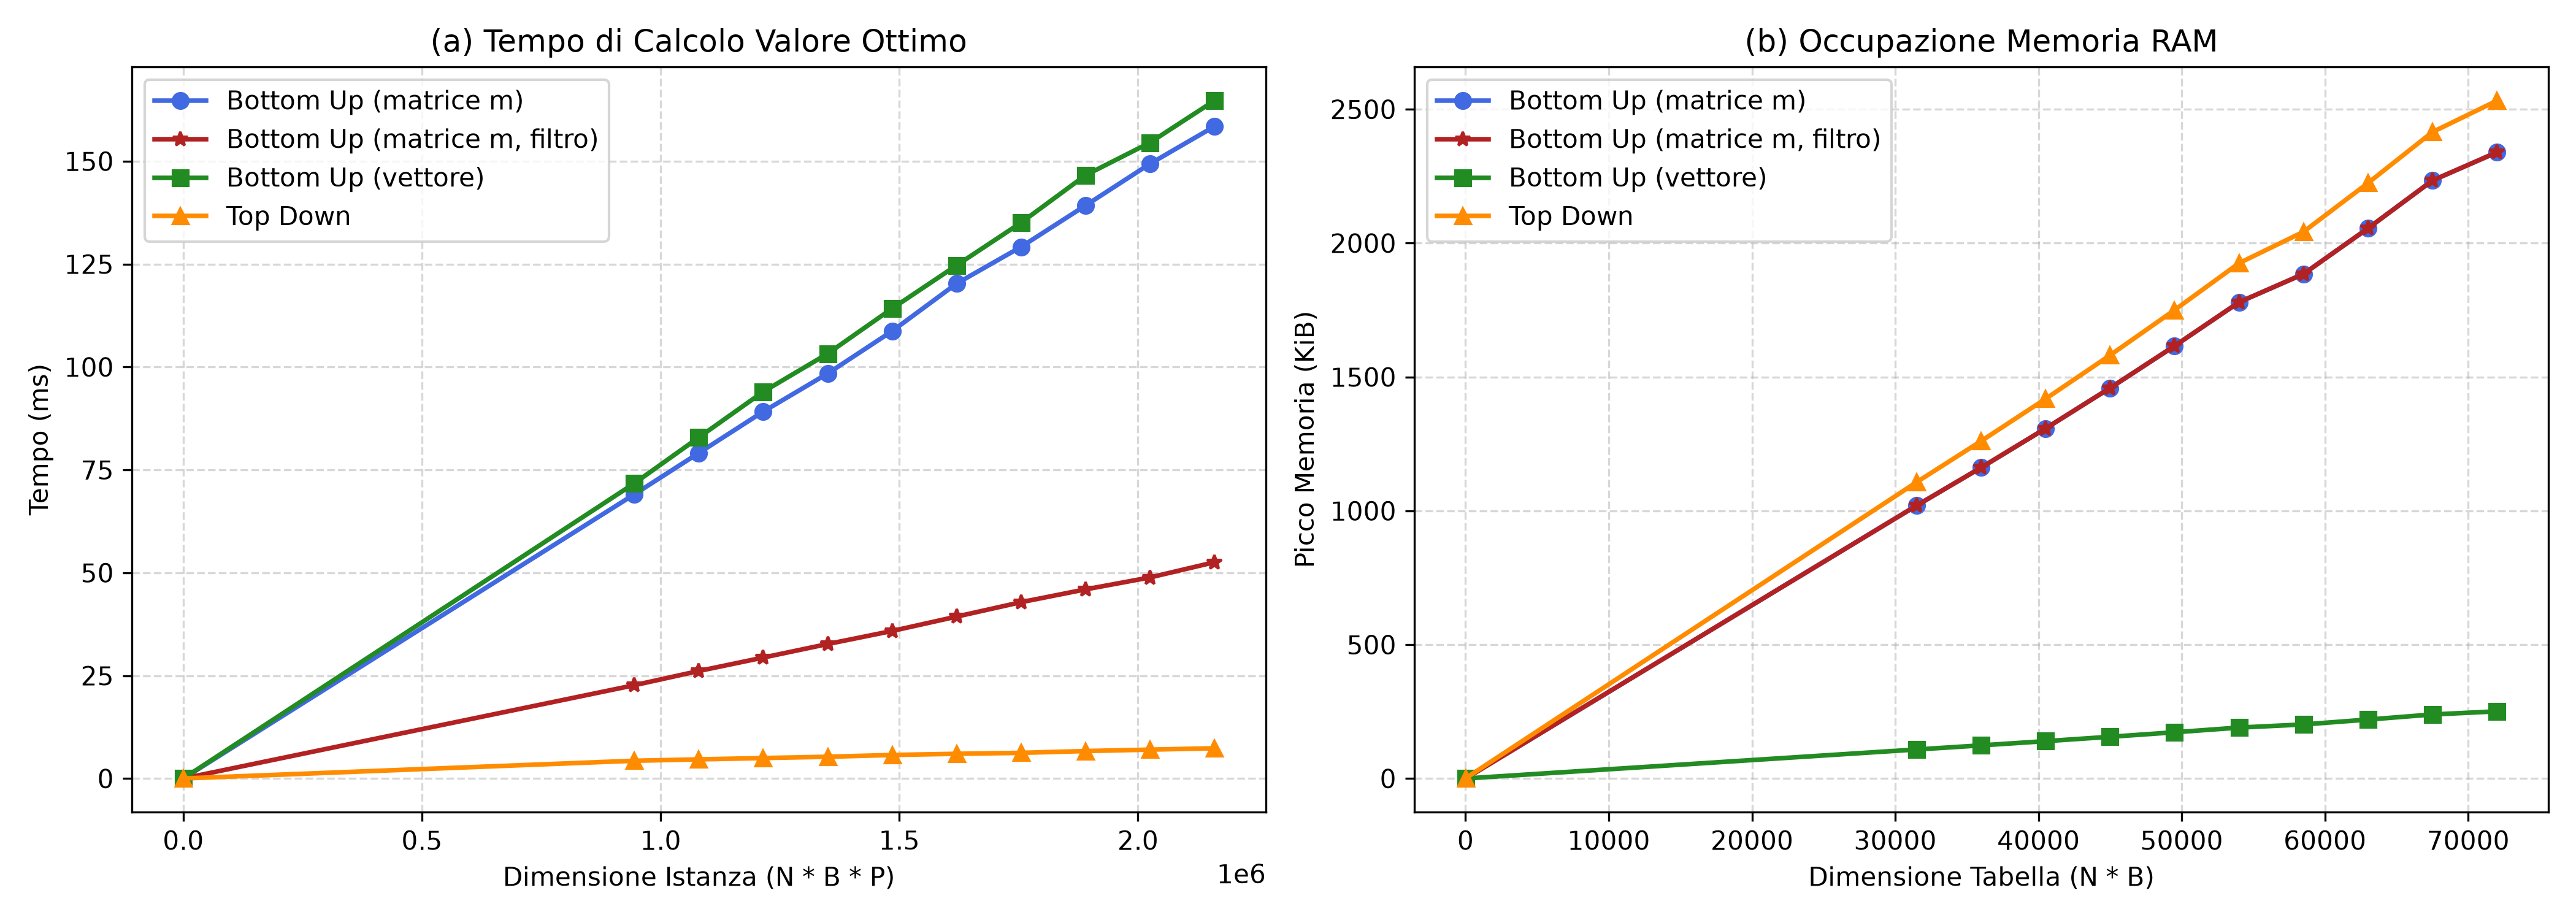
\includegraphics[width=\textwidth]{plot_optimal_value.png}
	\caption{Confronto delle prestazioni degli algoritmi: (a) tempo di calcolo rispetto alla dimensione dell'istanza ($N \cdot B \cdot P$); (b) picco di memoria rispetto alla dimensione della tabella ($N \cdot B$).}
	\label{fig:optimal_value_plots}
\end{figure}

All'aumentare del budget discreto $B$, i tempi di esecuzione del Bottom-Up base e delle sue varianti principali mostrano una crescita chiaramente lineare. Poiché il numero di ruoli $N = 9$ e il numero di candidati $P = 30$ sono mantenuti costanti in tutti gli scenari, la dimensione complessiva dell'istanza scala in modo direttamente proporzionale a $B$. Ad esempio, confrontando gli scenari estremi ($B = 3500$ e $B = 8000$), a fronte di una crescita del budget di circa $2.29$ volte si registra un incremento dei tempi di calcolo di circa $2.36$ volte, confermando fedelmente l'andamento previsto dall'analisi asintotica $O(N \cdot B \cdot P)$.

Un aspetto interessante riguarda il confronto tra il Bottom-Up su matrice e la variante a vettore singolo. Anche se quest'ultima opera su una sola riga anziché sull'intera tabella, il numero totale di controlli e aggiornamenti interni rimane identico. Per verificare questa equivalenza è stata calcolata la discrepanza percentuale tra i tempi:
\begin{equation}
	\Delta_{\text{time}}\% = \frac{T_{\text{vettore}} - T_{\text{matrice}}}{T_{\text{matrice}}} \times 100
\end{equation}
Su tutti i 10 scenari analizzati, la differenza media tra i tempi delle due versioni è di appena il $+4.99\%$; applicando il filtraggio preliminare scende addirittura all'$1.06\%$. Questa piccola differenza è del tutto trascurabile e dipende solo da dettagli interni di Python: la versione con matrice sfrutta la copia rapida di un'intera riga (\texttt{m[i][:] = m[i-1][:]}), mentre quella a vettore singolo compie un controllo condizionale (\texttt{if}) elemento per elemento. I dati confermano quindi che la variante a vettore singolo preserva integralmente la complessità temporale $O(N \cdot B \cdot P)$.

L'applicazione del filtro preliminare permette invece di ridurre notevolmente i tempi di calcolo mantenendo intatta la correttezza del risultato. Scartando in partenza i candidati dominati all'interno di ciascun ruolo, il numero effettivo di giocatori da valutare scende in media da $P = 30$ a circa $P' \approx 10$. Poiché il ciclo più interno compie un numero di iterazioni proporzionale a $P'$, il tempo di esecuzione si riduce di circa due terzi (rispecchiando il rapporto teorico $P'/P \approx 1/3$), consentendo un netto guadagno di velocità.

L'algoritmo Top-Down ricorsivo con memoizzazione si dimostra la soluzione più rapida in assoluto, con tempi inferiori di un ordine di grandezza rispetto agli approcci iterativi. Questo comportamento è dovuto alla natura discreta e sparsa dei costi dei contratti: scendendo a ritroso dallo stato finale $(N, B)$, gran parte delle celle $(i, b)$ della matrice non viene mai raggiunta da combinazioni valide di acquisti. Il Top-Down valuta esclusivamente gli stati strettamente necessari per risolvere l'istanza, evitando di riempire l'intera griglia $\Theta(N \cdot B)$ ed esplorando un numero di transizioni ampiamente inferiore al caso peggiore teorico $O(N \cdot B \cdot P)$.

\subsubsection{Occupazione di Memoria}
I valori di picco di memoria heap campionati tramite \texttt{tracemalloc} sono riportati nella Tabella~\ref{tab:memory_consumption} e mostrati graficamente nella Figura~\ref{fig:optimal_value_plots}(b).

\begin{table}[!htbp]
	\centering
	\small
	\caption{Picco di memoria heap allocata (in KiB) per gli algoritmi di calcolo del valore ottimo.}
	\label{tab:memory_consumption}
	\begin{tabular}{lccccc}
		\toprule
		\textbf{Scenario} & $B$ & \textbf{BU (con $s$)} & \textbf{BU (senza $s$)} & \textbf{BU (vettore 1D)} & \textbf{Top-Down} \\
		\midrule
		\texttt{sc\_01} & 3500 & 1306.0 & 1019.9 & 108.4 & 1107.2 \\
		\texttt{sc\_02} & 4000 & 1484.0 & 1161.6 & 123.7 & 1260.6 \\
		\texttt{sc\_03} & 4500 & 1670.7 & 1307.7 & 139.5 & 1418.5 \\
		\texttt{sc\_04} & 5000 & 1867.4 & 1458.8 & 155.8 & 1581.3 \\
		\texttt{sc\_05} & 5500 & 2076.0 & 1615.8 & 172.6 & 1750.0 \\
		\texttt{sc\_06} & 6000 & 2297.1 & 1779.1 & 190.1 & 1925.0 \\
		\texttt{sc\_07} & 6500 & 2402.6 & 1884.6 & 201.9 & 2042.2 \\
		\texttt{sc\_08} & 7000 & 2638.1 & 2055.0 & 220.1 & 2224.4 \\
		\texttt{sc\_09} & 7500 & 2889.8 & 2233.6 & 239.1 & 2414.7 \\
		\texttt{sc\_10} & 8000 & 2995.2 & 2339.1 & 250.8 & 2531.9 \\
		\bottomrule
	\end{tabular}
\end{table}

Il risultato più evidente è il forte calo di memoria ottenuto con la variante a vettore singolo, che fa registrare una riduzione dell'occupazione di circa il $90\%$ rispetto alla matrice completa $m$ (e di oltre il $91\%$ rispetto alla versione con entrambe le matrici $m$ ed $s$). Questo andamento rispecchia fedelmente il vantaggio teorico della variante: eliminando la necessità di allocare l'intera griglia bidimensionale e operando su un unico vettore di dimensione $B + 1$ aggiornato a ritroso, l'algoritmo cancella la dipendenza dal numero di ruoli $N$, riducendo la complessità spaziale da $\Theta(N \cdot B)$ a $\Theta(B)$.

Per quanto riguarda il Top-Down, l'occupazione di memoria segue da vicino il profilo del Bottom-Up senza matrice ausiliaria $s$, condividendo la medesima classe di complessità spaziale $\Theta(N \cdot B)$. Per comprendere questo andamento è utile distinguere tra la memoria allocata sull'heap e quella impegnata sullo stack delle chiamate ricorsive:
\begin{itemize}
	\item \textbf{Memoria heap:} per memorizzare i risultati dei sottoproblemi, l'algoritmo crea all'avvio l'intera tabella \texttt{memo} di $(N+1) \times (B+1)$ elementi con valori sentinella negativi. Poiché \texttt{tracemalloc} rileva lo spazio totale allocato per le strutture dati sull'heap, l'ingombro riflette la dimensione complessiva della matrice dinamica $\Theta(N \cdot B)$, anche se molte celle non vengono effettivamente calcolate durante l'esplorazione.
	\item \textbf{Stack di ricorsione:} ogni chiamata di funzione aggiunge un record di attivazione sullo stack di Python. Tuttavia, poiché a ogni passo si passa al ruolo precedente ($i \to i-1$), la profondità massima della ricorsione è limitata a $N = 9$ chiamate annidate. Lo spazio occupato dallo stack è quindi limitato a $O(N)$ record, una quantità del tutto trascurabile rispetto al costo $\Theta(N \cdot B)$ della tabella presente sull'heap.
\end{itemize}

\subsubsection{Ricostruzione della Rosa e Verifica dei Risultati}
È stato verificato che le diverse strategie di ricostruzione producano la stessa soluzione ottima. Su tutti i 10 scenari analizzati, la ricostruzione basata sulla matrice decisionale $s$ e quella eseguita direttamente sulla matrice dei valori $m$ identificano esattamente la stessa combinazione di giocatori, confermando la piena correttezza della risalita senza matrice ausiliaria e producendo sempre lo stesso valore ottimo con la copertura di tutti i 9 ruoli previsti.

\begin{figure}[!htbp]
	\centering
	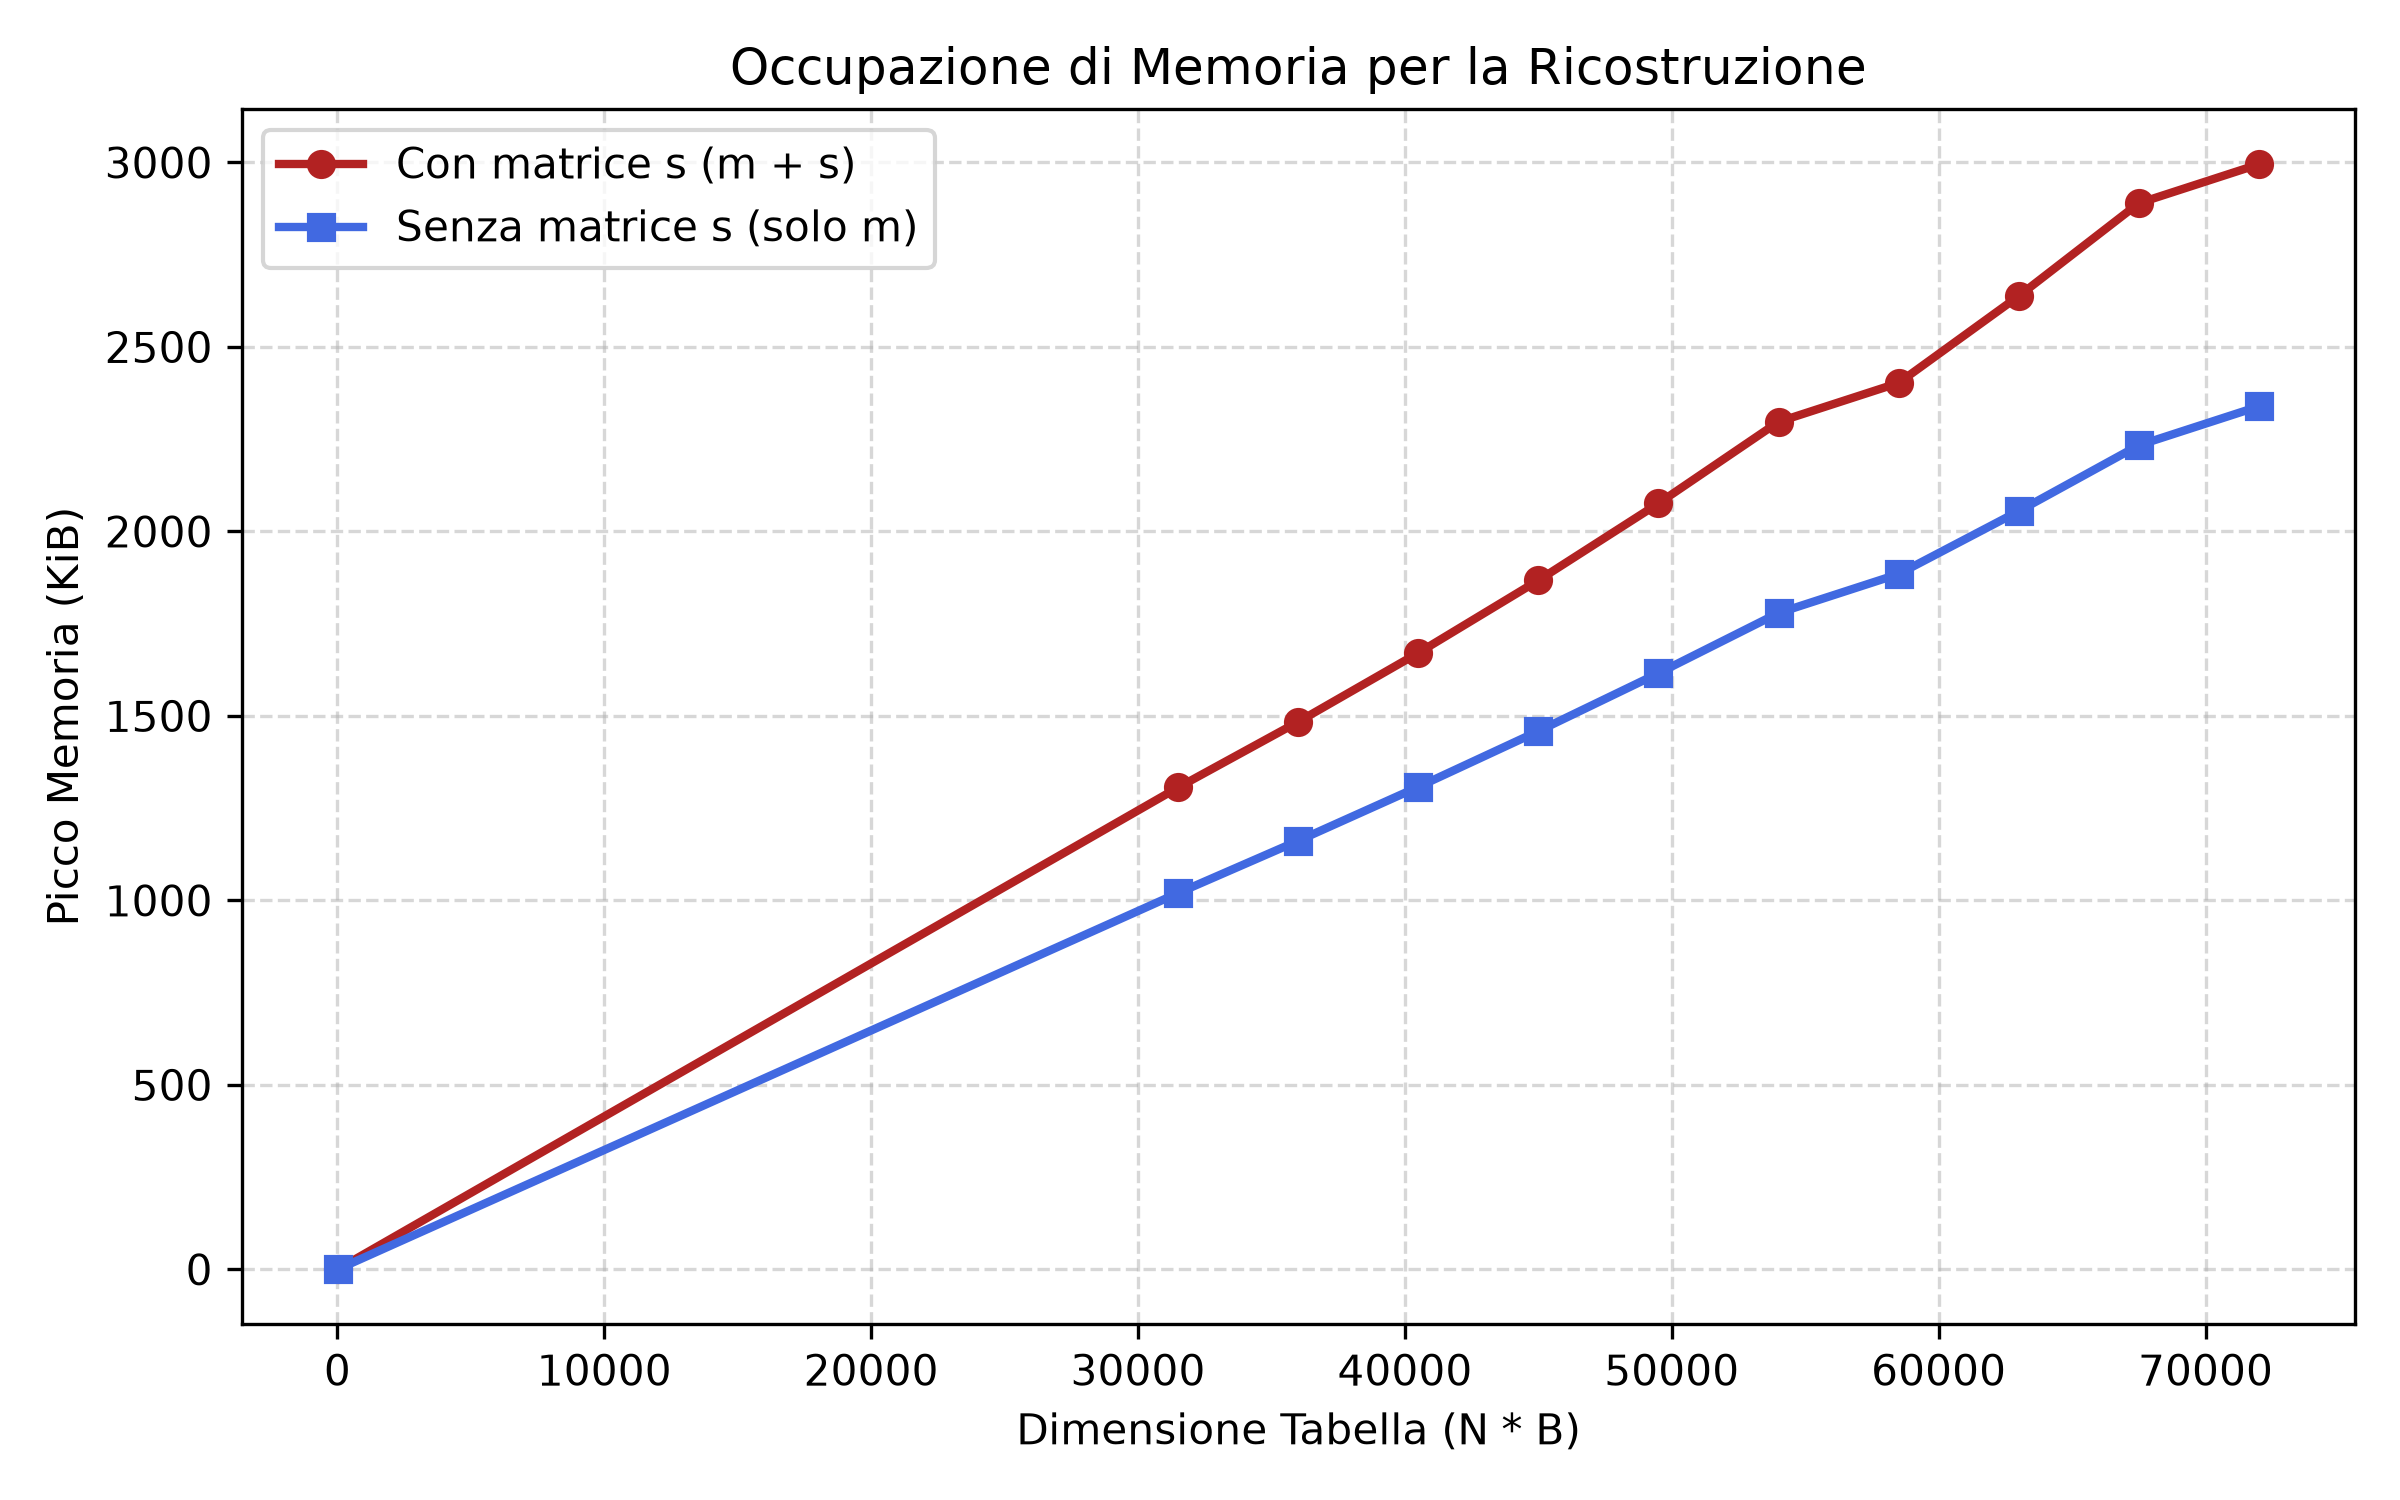
\includegraphics[width=0.72\textwidth]{plot_reconstruction_memory.png}
	\caption{Confronto dell'occupazione di memoria heap tra la strategia con matrice delle decisioni $s$ e la strategia con sola matrice $m$.}
	\label{fig:reconstruction_memory_plot}
\end{figure}

Come mostrato nella Figura~\ref{fig:reconstruction_memory_plot}, la scelta del metodo di ricostruzione comporta un chiaro compromesso tra tempo di esecuzione e memoria occupata:
\begin{itemize}
	\item \textbf{Ricostruzione con matrice $s$:} consente di estrarre la formazione in tempo lineare $\Theta(N)$, ma richiede di mantenere in memoria entrambe le matrici $m$ ed $s$ durante tutto il calcolo dinamico, impiegando complessivamente $2(N+1)(B+1)$ celle e raddoppiando la memoria allocata.
	\item \textbf{Ricostruzione senza matrice $s$:} ricostruisce la soluzione a ritroso controllando direttamente la matrice $m$ in tempo $O(N \cdot P)$. In cambio, permette di dimezzare l'occupazione di memoria allocando solo la matrice $m$ da $(N+1)(B+1)$ elementi.
\end{itemize}

\newpage

\section{Guida all'Uso e Conduzione di Ulteriori Sperimentazioni}

Questa sezione fornisce le indicazioni operative necessarie alla configurazione dell'ambiente, all'esecuzione degli algoritmi realizzati e all'ispezione delle tabelle prodotte, illustrando inoltre le linee guida per la conduzione di ulteriori sperimentazioni su nuove istanze del problema.

\subsection{Requisiti e Configurazione dell'Ambiente}
Il software sviluppato richiede un interprete Python in versione 3.10 o successiva. Le librerie esterne necessarie all'esecuzione sono elencate nel file \texttt{requirements.txt} e comprendono: \texttt{numpy}, \texttt{pandas} e \texttt{matplotlib}.

Per predisporre l'ambiente di esecuzione isolato, si consiglia la creazione di un ambiente virtuale dedicato tramite i comandi:

\noindent\begin{minipage}{\linewidth}
\begin{verbatim}
# Creazione dell'ambiente virtuale
python3 -m venv .venv

# Attivazione dell'ambiente virtuale
# Su sistemi Unix/Linux e macOS:
source .venv/bin/activate
# Su sistemi Microsoft Windows (Prompt dei comandi):
.\.venv\Scripts\activate.bat
# Su sistemi Microsoft Windows (PowerShell):
.\.venv\Scripts\Activate.ps1

# Installazione delle librerie richieste
pip install -r requirements.txt
\end{verbatim}
\end{minipage}

\subsection{Modalità di Esecuzione}
Il programma principale del progetto è \texttt{demo.py}, che permette sia di eseguire i calcoli su tutti gli scenari generando i risultati, sia di mostrare le tabelle e la rosa ottima. È inoltre disponibile lo script \texttt{main.py} per eseguire i test in modo automatico da terminale.

\subsubsection{Demo e Sperimentazione}
Al fine di garantire la massima portabilità tra sistemi operativi differenti, nella radice del progetto sono stati predisposti specifici script di lancio automatico della demo:
\begin{itemize}
	\item \textbf{Sistemi Unix/Linux e macOS:} tramite lo script Bash \texttt{./run\_demo.sh} (previa assegnazione dei permessi di esecuzione con \texttt{chmod +x run\_demo.sh});
	\item \textbf{Sistemi Microsoft Windows:} tramite lo script batch \texttt{run\_demo.bat} (avviabile da riga di comando o direttamente dall'interfaccia grafica);
	\item \textbf{Invocazione standard Python:} mediante il comando \texttt{python demo.py} (o \texttt{python3 demo.py}).
\end{itemize}

All'avvio, il programma mostra una schermata articolata in due fasi:
\begin{enumerate}
	\item \textbf{Fase di calcolo ed elaborazione degli scenari:} il programma richiede se avviare la sperimentazione completa. Rispondendo affermativamente, il software elabora in sequenza tutti gli undici scenari presenti nella cartella \texttt{scenarios/}, eseguendo per ciascuno le sei varianti algoritmiche su $K = 15$ iterazioni, misurando tempi e picchi di memoria tramite \texttt{tracemalloc}, salvando le metriche in \texttt{results/benchmark\_metrics.csv}, esportando le tabelle dinamiche CSV e generando in automatico i tre grafici PNG di sintesi prestazionale. Qualora i risultati siano già stati calcolati in precedenza, l'utente può saltare tale fase per accedere istantaneamente ai dati già archiviati.
	\item \textbf{Fase di esplorazione interattiva:} conclusa la fase precedente, si apre il menu principale che offre cinque voci:
	\begin{itemize}
		\item \textbf{Opzione 1 (Mostra rosa ottimale):} visualizza in formato tabellare la rosa ottimale identificata dall'algoritmo di ricostruzione per lo scenario selezionato, con i dettagli di costo e rendimento per ciascun ruolo, accompagnata da un riepilogo (WAR totale, spesa sostenuta e budget residuo);
		\item \textbf{Opzione 2 (Visualizza tabelle):} permette di ispezionare a video le matrici $m$ ed $s$. Nelle istanze compatte (come lo scenario demo), le tabelle vengono stampate integralmente, mentre nelle istanze con budget elevato viene mostrata una visualizzazione compatta composta dalle prime 4 colonne, da una colonna di separazione e dalle ultime 4 colonne. In entrambi i casi, viene evidenziato il valore ottimo $m[N, B]$;
		\item \textbf{Opzione 3 (Confronta le varianti algoritmiche):} esegue in tempo reale sullo scenario corrente tutte le sei varianti, stampando una tabella comparativa che certifica la perfetta uguaglianza del valore ottimo calcolato ed esplicita quali varianti supportano la ricostruzione della rosa e quali si limitano al calcolo del solo valore;
		\item \textbf{Opzione 4 (Cambia scenario):} permette di cambiare lo scenario attivo selezionandolo dall'elenco di quelli disponibili;
		\item \textbf{Opzione 5 (Grafici e benchmark delle prestazioni):} rimanda a un sotto-menu che mostra altre voci per la visualizzazione dei grafici generati.
	\end{itemize}
\end{enumerate}

\subsubsection{Ispezione delle Tabelle Generate}
Per la visualizzazione integrale delle tabelle, nei casi in cui il budget assuma dimensioni realistiche rendendo impossibile una lettura a schermo, è possibile consultare i file generati nella cartella \texttt{results/}:
\begin{itemize}
	\item \texttt{matrice\_m\_<scenario>.csv}: contiene la matrice bidimensionale dei valori WAR, con intestazioni di riga associate a ciascun ruolo e intestazioni di colonna relative al budget discretizzato $b \in \{0, \dots, B\}$;
	\item \texttt{matrice\_s\_<scenario>.csv}: contiene la matrice bidimensionale delle scelte, in cui ogni cella $s[i, b]$ riporta l'indice $j \ge 0$ del candidato ingaggiato o il valore convenzionale $-1$ qualora per il ruolo $i$ non sia stato selezionato alcun giocatore.
\end{itemize}

\subsection{Conduzione di Ulteriori Sperimentazioni}
Il software è progettato per consentire la sperimentazione su nuove istanze, variando sia le caratteristiche dimensionali sia i parametri di campionamento.

\subsubsection{Formato dei Dati di Ingresso}
Le nuove istanze del problema devono essere codificate in file con estensione \texttt{.json} e collocate all'interno della cartella \texttt{scenarios/}. La struttura sintattica attesa dal modulo di caricamento (\texttt{src/core/loader.py}) è la seguente:

\noindent\begin{minipage}{\linewidth}
\begin{verbatim}
{
  "scenario_name": "scenario_personalizzato",
  "budget": 500000000,
  "cost_unit": 100000,
  "roles": [
    {
      "role_name": "Pitcher",
      "candidates": [
        { "name": "Player A", "cost": 15000000, "war": 4.5 },
        { "name": "Player B", "cost": 10000000, "war": 3.8 }
      ]
    }
  ]
}
\end{verbatim}
\end{minipage}
Il modulo calcola automaticamente la dimensione dell'istanza e ordina gli scenari in base alla complessità prima dell'esecuzione dei test.

\subsubsection{Linee Guida per Ulteriori Sperimentazioni}
Per estendere la sperimentazione oltre la variazione del budget, il software permette di testare nuove configurazioni modificando semplicemente i parametri nei file JSON:
\begin{itemize}
	\item \textbf{Variazione dei ruoli ($N$):} testando istanze con un numero di ruoli diverso da $N = 9$ (tipico del baseball), è possibile verificare che tempo e memoria crescano in modo lineare, coerentemente con le complessità teoriche $O(N \cdot B \cdot P)$ e $\Theta(N \cdot B)$;
	\item \textbf{Variazione dei candidati ($P$):} modificando il numero di giocatori per ruolo si può confermare che l'occupazione di memoria resta costante (essendo indipendente da $P$) e analizzare l'efficacia del filtro, che scarta una quota percentuale maggiore di giocatori dominati quando il numero di candidati aumenta.
\end{itemize}

\newpage

\section{Limitazioni Riscontrate}
Durante la realizzazione del progetto e l'analisi dei risultati sperimentali sono emerse alcune limitazioni pratiche, legate sia al modello teorico sia alle scelte implementative adottate:

\begin{itemize}
	\item \textbf{Dipendenza dal budget:} La complessità degli algoritmi dipende direttamente dal valore numerico del budget $B$. Avendo impostato la scala a $100\,000$ dollari ($\text{COST\_UNIT} = 100\,000$), $B$ rimane nell'ordine di qualche migliaio e i tempi di esecuzione restano inferiori al secondo. Se però si volesse una precisione al singolo dollaro per gestire cifre contrattuali esatte, $B$ salirebbe a centinaia di milioni: in quel caso la tabella dinamica diventerebbe del tutto ingestibile, rendendo i tempi di calcolo proibitivi ed esaurendo rapidamente la memoria RAM.

	\item \textbf{Vettore singolo e impossibilità di ricostruire la rosa:} La variante a vettore singolo consente un notevole risparmio di memoria, ma presenta il limite di non poter ricostruire la rosa ottimale. Poiché l'unico array viene sovrascritto a ogni ruolo, alla fine dell'esecuzione si ottiene unicamente il valore del WAR massimo raggiungibile, perdendo la traccia di quali giocatori siano stati effettivamente acquistati. Questa variante è quindi utilizzabile solo quando interessa il valore numerico della soluzione e non l'elenco dei candidati selezionati.

	\item \textbf{Efficacia del filtro legata alla distribuzione dei candidati:} Il filtro preliminare è risultato molto efficace sugli scenari, riducendo i candidati da 30 a circa 10 per ciascun ruolo, perché nei dati di partenza erano presenti molti candidati svantaggiosi (con costo elevato e WAR ridotto). Tuttavia, il beneficio del filtro dipende interamente dai dati: se tutti i giocatori con costo maggiore avessero anche un WAR strettamente superiore, il filtro non riuscirebbe a scartare nessuno, introducendo soltanto il tempo aggiuntivo necessario a ordinare le liste.

	\item \textbf{Gestione delle parità e soluzioni ottime multiple:} Gli algoritmi aggiornano la soluzione solo quando trovano un valore strettamente superiore (\texttt{war > m[i][b]}). Se ci sono più giocatori con lo stesso costo e lo stesso rendimento, il programma ne seleziona deterministicamente solo uno (il primo incontrato). Gli algoritmi non sono quindi strutturati per enumerare o mostrare tutte le rose ottimali alternative equivalenti, ma ne restituiscono sempre una singola.
\end{itemize}

\newpage


\end{document}
